\documentclass[a4paper, xelatex, ja=standard]{bxjsarticle}
% \setpagelayout*{top=25truemm,bottom=25truemm,left=25truemm,right=25truemm}

% パッケージインストール
\usepackage{plisting}
\usepackage{docmute}

% 文書開始
\begin{document}
\maketitle
\begin{abstract}
Ray Tracing in One Weekend(週末レイトレーシング)
と言うサイトでは,
レイトレーシングをC++で
簡単に実装する方法について解説されている.
その中では当たり前だが多少の計算が必要で,
プログラミングやレイトレーシングに興味を持った未来の高専生たちが,
いざ作ってみようと思っても(コード例が載っているので作ることはできるが)
完全に理解した状態で作るには説明が足りないと思われる.
そこでその計算方法やその他屈折に関する興味深い事実をまとめた.
\end{abstract}

\section{はじめに}
最近のゲームや映画の映像は
ものによっては現実と区別がつかないほど
高度な域にまで達している(特に金属や機械など).
商業的に使われているものほど複雑なものは難しいが,
単純な金属球やガラス球といったものを
現実のような美しさで1から描画するのは
実はさほど難しくない.

レイトレーシングという3D CGの描画手法を使えば
(プログラミングを実行できる環境を持っていれば)
誰でも簡単に以下のような画像を生成させることができる.
\begin{figure}[b]
\centering
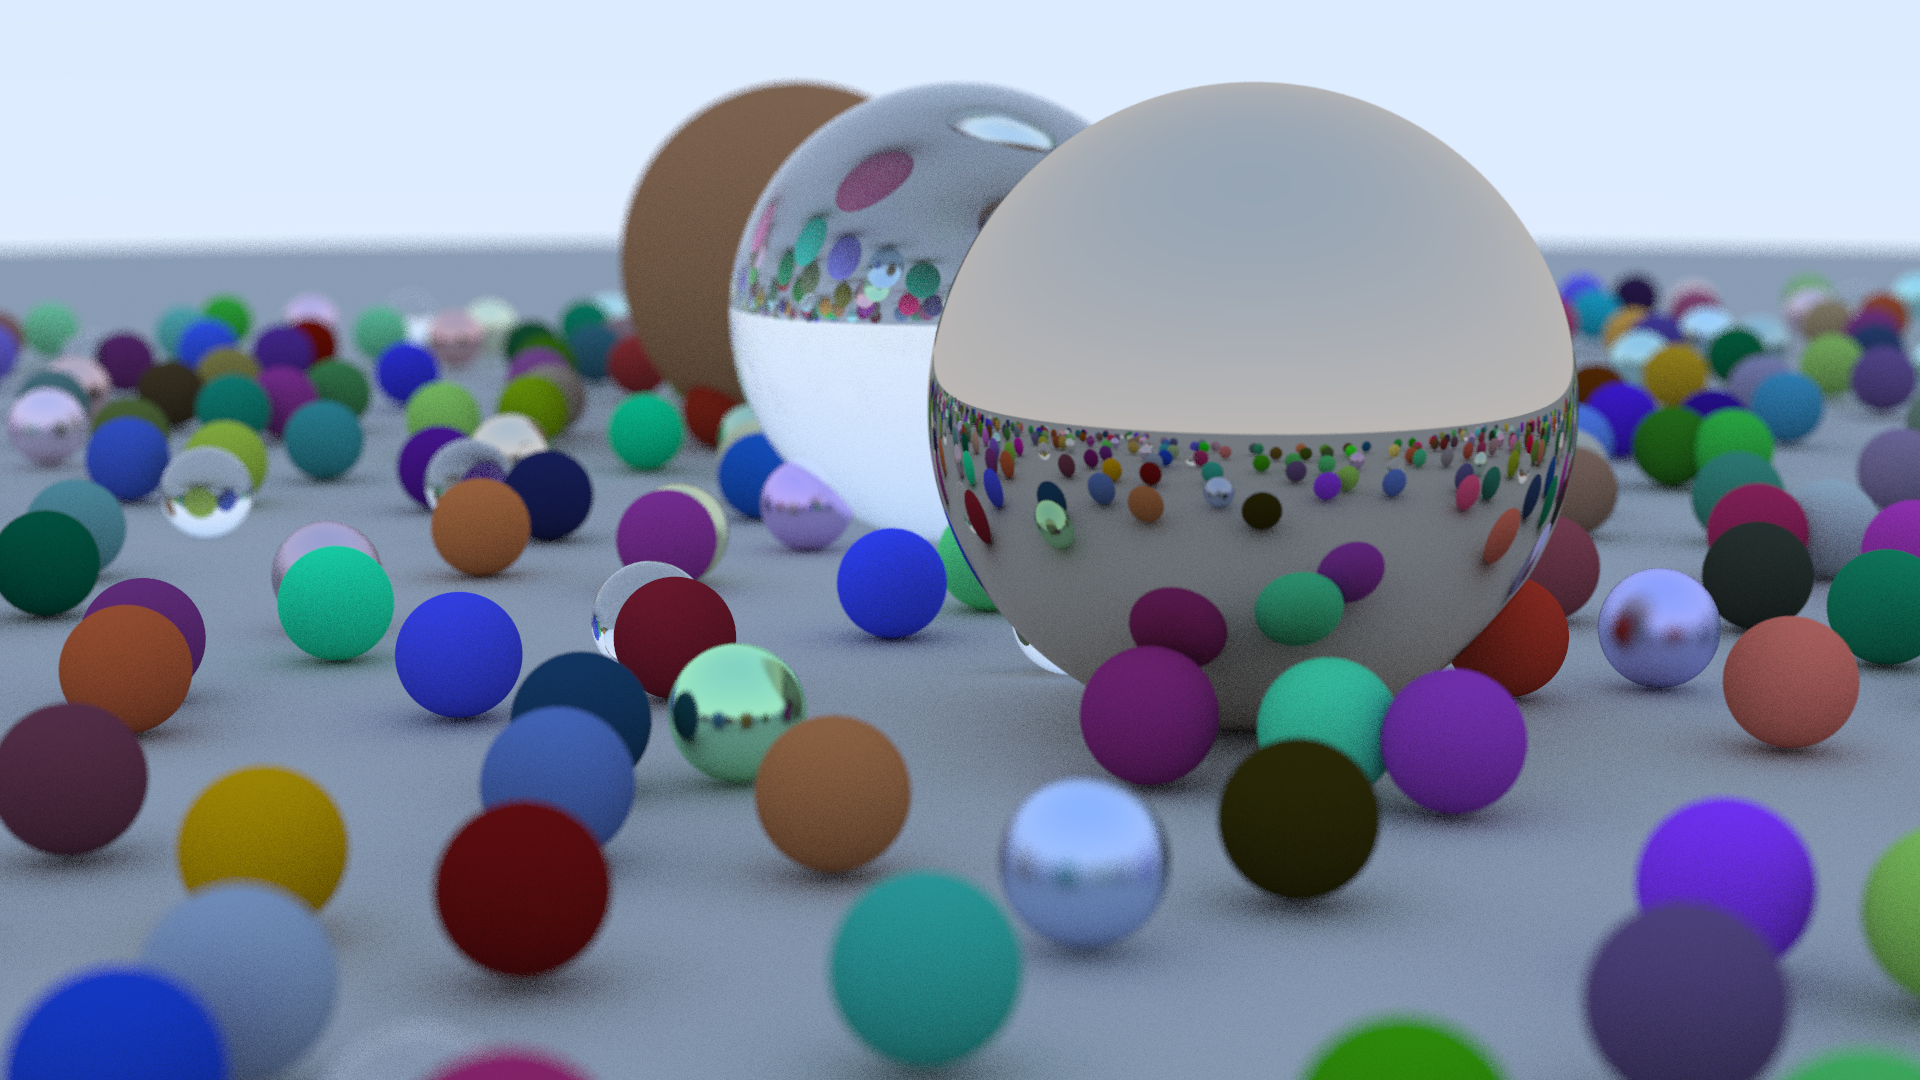
\includegraphics[scale=0.2]{img/example.png}
\caption{実際に描画した画像}
\label{}
\end{figure}
印刷の関係で白黒になっているだろうが
美しい画像を生成できることは確認できるだろう.
念を押すが誰でもBlenderやUnreal Engineといった
ソフトウェアを使わずに3D CGを描画できるのだ.

こちらではこれの作り方は説明しない.
既にRay Tracing in One Weekendというサイト
で作り方を無料公開しているからだ.
こちらではそのサイトでは説明不足に感じた
光の屈折の計算方法とそれに関する蛇足情報をまとめてある.
まず計算する際に必要になる知識の説明をする.

\section{必要になる知識の説明}
\subsection*{三角比}
\begin{figure}[h]
\centering
\begin{tikzpicture}[scale=2]
    \coordinate(A)at({sqrt(3)}, 1);
    \coordinate(B)at(0, 0);
    \coordinate(C)at({sqrt(3)}, 0);
    
    \draw(A)node[above]{$\mathrm{A}$};
    \draw(B)node[left]{$\mathrm{B}$};
    \draw(C)node[right]{$\mathrm{C}$};
    
    \draw(A)--(B)--(C)--(A);
\end{tikzpicture}
\caption{直角三角形}
\label{fig:sin-triangle}
\end{figure}

図\ref{fig:sin-triangle}のような直角三角形がある.
$\angle\mathrm{ABC}=\theta$とする.
それぞれ向かい合う辺を$a, b, c$とすると
三角比は以下のように定義される.
\[
\sin{\theta}=\frac{b}{c}\hspace{5mm}
\cos{\theta}=\frac{a}{c}\hspace{5mm}
\tan{\theta}=\frac{b}{a}
\]
なお今回使うのは$\sin$だけである.
また定義から明らかなことではあるが
斜辺の長さをかければそれぞれ高さ, 底辺の長さ
を求めることができる.

\subsection*{ベクトル}
今まで使ってきた長さや速さといったものは
1つの値で表してきた.
このようなものをスカラーと言う.
これに方向といった情報を追加し,
複数の値を使って表すものをベクトルという.
$\vec{a}$や$\vb{a}$などを使う.
今回は後者を使う. 格好良いから.
ベクトルの演算方法については,
加算, 内積, 大きさの計算方法がわかっていれば良いので, 
その3つについて説明する.

加算については図\ref{fig:vector-add}のようなイメージを持ってもらえば良い.
マイナスがついた場合方向が真逆になると思って欲しい.
\begin{figure}[h]
\centering
  \begin{tikzpicture}[scale=1]
  \coordinate(A)at(0,0);
  \coordinate(B)at(2,1);
  \coordinate(C)at(4,-1);

  \draw[-Stealth, thick](A)--node[above left]{$\vb{a}$}(B);
  \draw[thick](B)--node[above right]{$\vb{b}$}(C);
  \draw[-Stealth, thick](A)--node[below]{$\vb{a}+\vb{b}$}(C);
  \end{tikzpicture}
\caption{ベクトルの加算}
\label{fig:vector-add}
\end{figure}

内積は2つのベクトル$\vb{a, b}$のなす角を$\theta$とするとき
以下のように定義される.
\[
\vb{a}\cdot\vb{b}=|\vb{a}||\vb{b}|\cos{\theta}
\]
$|\vb{a}|$は$\vb{a}$の大きさを意味しており,
$\theta$は$\vb{a}$と$\vb{b}$のなす角度である.
イメージとしては$\vb{a}$の終端から
$\vb{b}$へ垂線をおろし, その長さに
それぞれの大きさ(長さ)をかけたものだ.
式を見ればわかることだが内積で得られる値はスカラーである.

\section{光の屈折とは}
光が別の物質へ入るとき(入射),
光が曲がる現象がある.
これを屈折という.
水面に景色が映り込んだり,
分厚いガラスから見る景色が歪んでいたりするのは
この屈折という現象によって引き起こされる.

\subsection{屈折のメカニズム}
そもそも屈折とはどのようにして起きるのだろう.
図\ref{fig:light-refraction}に屈折する光の簡単なモデルを載せた.
\begin{figure}[h]
\centering
  \begin{tikzpicture}[scale=0.3]
  % \coordinate(A)at(0,0);
  % \coordinate(B)at(2,1);
  % \coordinate(C)at(4,-1);

  % \draw[-Stealth, thick](A)--node[above left]{$\vb{a}$}(B);
  % \draw[thick](B)--node[above right]{$\vb{b}$}(C);
  % \draw[-Stealth, thick](A)--node[below]{$\vb{a}+\vb{b}$}(C);
  \coordinate(A)at(0, 3);
  \coordinate(B)at(0, 0);
  \coordinate(C)at(0, -3);
  \draw[thick](0, 7)--(0, -7);

  \draw[dashed](A)--(-5, 2);
  \draw[dashed](A)--(5, 7);
  \draw[dashed](B)--(-5, -1);
  \draw[dashed](B)--(5, 4);
  \draw[dashed](C)--(-5, -4);
  \draw[dashed](C)--(5, 1);

  \draw[-Stealth, thick]({-15/26-5/2},{75/26-1/2})--({-5/2}, {-1/2});
  \draw[-Stealth, thick]({-60/41+5/2},{75/41+4/2-3})--({5/2}, {4/2-3});
  \end{tikzpicture}
\caption{屈折のモデル}
\label{fig:light-refraction}
\end{figure}
光は波の性質を持っているので,
図\ref{fig:light-refraction}の破線は光の波の山の位置を描いており,
矢印は光の山と山の距離, 波長の長さだけ引いてある
(山と山の最短距離=波長).
光が他の物質に入るときに曲がるのであれば,
必然的に図\ref{fig:light-refraction}のように波の方向が変化する.
このとき, 山の接触しなければ波の周期にずれが起きてしまうので,
波の方向を変えると一緒になって波の間隔も短くなる.

光の波長が変わったとしても
光の波から波までの時間, 周期は変わってしまっては
おかしなことになる.
なぜなら元は同じ光源だったはずだからである.
であれば波長を変えるには速さを変えるしか方法はない(\ref{eq:wave}).
よって屈折とは光が他の物質へ入射する際に
速度が変わることによって引き起こされることがわかった.

\begin{equation}
\lambda=vT (\lambda:\mbox{波長}v\mbox{:速度}T:\mbox{周期})\label{eq:wave}
\end{equation}

\subsection{光が遅くなるとは}
この宇宙で最速の光くんは"真空中"で
速度$c\simeq 300,000\si{km/s}$とされている.
これは1秒で地球を7周半できるほどの速さである
\footnote{速い, が宇宙の最速としては遅い, と思う}.
なぜ"真空中で"となっている理由は先程説明した.

しかし光速というものは同時に絶対的であるとも言われている.
どんな状態(速さ)から見ても光の速度は変化しない.
そのため時間が伸び縮みするのだが
そんなことを言っておきながら光が遅くなってどうすんだと思うだろう.
実は物質中では光は遅くなるというのは
半分嘘である.
正しくは"見かけ上"光は光速$c$より遅くなるのだ.

ここからはある程度数式を使って
小難しいことを言っているが,
正直式の内容を理解しなくても
文章の部分が理解できれば十分だ.

まず電場, 電磁波について簡単に話そう.
この世のありとあらゆる物質はすべて原子からできており,
原子は原子核とその周りにある電子で構成されている.
その原子核には陽子という正の電荷(電気)を持つものと
電荷を持たない中性子がある.
こいつらも分解できるがこの話には関係ないので割愛する.

ここで今回重要になってくるのは電荷を持つ
電子と陽子だ.
陽子に関しては単体であることはほとんどないので
原子核として考えてよいだろう.
これらは存在するだけで電場と呼ばれる空間を作り,
この電場の強さや様々な電場が重ね合わさることによって生じる
向きに従って, 電荷を持つ物質は力を加えられる
\footnote{電荷からの距離と電場を生み出している電荷の大きさによって
電場の強さは変化し, それらは異符号の電荷を自身に引き寄せるような力が働いている.
世界中に電荷を持つ物体は大量にあるので, 複雑に絡みあうのだ.
中学生であれば磁力線のようなものだと思って欲しい.}.
丁度電気がプラスからマイナスに流れるような感じだ.

さてこの電場は光速$c$で伝わる.
また電場は電荷を持つ物質との距離にも依存するので
もし電荷が移動すれば電場に変化が生まれることになる.
これが電磁波となって伝わるのだ
\footnote{少々雑な説明なので注意してください}.

さてここからは簡単な数式を使いながら説明する.
まず状況を設定する.
薄いガラスの板があり,
横から見て左の遠くに外部光源$S$があり,
右の遠くにある観測点$P$での電場について考える.
\begin{figure}[h]
\centering
  \begin{tikzpicture}[scale=1]
  \coordinate(G1)at(-0.1, 1);
  \coordinate(G2)at(0.1, 1);
  \coordinate(G3)at(0.1, -1);
  \coordinate(G4)at(-0.1, -1);
  \draw(G1)--(G2)--(G3)--node[below]{glass}(G4)--(G1);

  \coordinate(S)at(-7, 0);
  \draw[-Stealth, dashed](S)--node[above]{$\vb{E}_s$}(-3, 0);
  \fill[white](S)circle[radius=0.05]node[below]{$S$};
  \draw(S)circle[radius=0.05]node[below]{$S$};

  \coordinate(P)at(7, 0);
  \fill[black](P)circle[radius=0.05]node[below]{$P$};
  \end{tikzpicture}
\caption{問題設定}
\label{fig:light-refraction}
\end{figure}
まず$P$における電場を求めるが,
$S$の発する電磁波がガラスの板の原子にある
電子にも作用し電場が変化する.
結果$P$における電場も$S$からの電磁波による影響以外に
様々な影響を受けることになる.
もちろんこの宇宙の全電荷による作用もあるが
今回の場合はそれらは無視できるほど小さいものと仮定する.
ではこの仮定を元に
$P$における電場を$\vb{E}$,
$S$の発する電場を$\vb{E}_s$,
ガラス板内の振動する電荷による電場を$\vb{E}_a$とすると以下のようになる.
\begin{equation}
\vb{E}=\vb{E}_s+\vb{E}_a
\end{equation}

ここからははこの$\vb{E}_a$がどうなるのかを考えていく.
まずはじめに単純に屈折率$n$の物質中を進む光の速さは
$\frac{c}{n}$になるとする.
もしガラス板が何の影響も持たないとすると,
右($z$軸)に進む波の電場は
\begin{equation*}
E_s=E_0\cos{\omega\left(t-\frac{z}{c}\right)}
\end{equation*}
となる.
オイラーの公式
\footnote{$e^{i\theta}=\cos{\theta}+i\sin{\theta}$}
を用いると以下のように表すこともできる.
\begin{equation*}
E_s=E_0e^{i\omega\frac{t-z}{c}}
\end{equation*}
$i$は虚数単位なので$\sin$の部分は情報として落ちるので問題ない.
$z$は$S$と$P$の距離を表している.
$\cos$については先程説明したのでなんとなくわかると思うが,
これは波を表すことになる.
時間に関係してくるため$t$が入っており,
また距離を速さで割った$\frac{z}{c}$だけ
伝わる時間に差ができる.
なぜならこの$E_s$というのは$S$での電場であり
$t$は$P$を基準に決めているからである.

ここで板厚を$\Delta z$とすると
板が無ければこの距離を
$\frac{\Delta z}{c}$の時間で進むが,
仮に



\section{屈折光の計算}
実際に屈折光をスネルの法則を中心に計算していくが
計算過程でいくつか高校数学で習うものを使う.
といってもちょろいので簡単な説明をしておく.

\subsection{スネルの法則}
先程まで屈折率を$n$で扱ってきたが
諸事情(法線を$\vb{n}$で表したい)により
屈折率を$\eta, \eta'$で表す.
ここで使う記号を以下にまとめる.
なおベクトルは全て単位ベクトルである.
\begin{table}[h]
  \centering
  \caption{記号の意味}
  \label{}
  \begin{tabular}{c|c}
  名前 & 意味 \\\hline
  $\eta$ & 入射側の屈折率 \\
  $\eta'$ & 屈折側の屈折率 \\
  $\theta$ & 入射角 \\
  $\theta'$ & 屈折角 \\
  $\vb{n}$ & 法線のベクトル \\
  $\vb{R}$ & 入射光 \\
  $\vb{R'}$ & 反射光 \\
  $\vb{R'}_\parallel$ & 反射光の法線に平行な成分 \\
  $\vb{R'}_\perp$ & 反射光の法線に垂直な成分 \\
  \end{tabular}
\end{table}

まず屈折の法則としてスネルの法則を載せる.
これが屈折光を求める上での基本となる.
スネルの法則の導出についてはGoogle先生に聞けば一発なので
気になる場合は各自調べてほしい.
\begin{equation}
\eta\cdot\sin{\theta}=\eta'\sin{\theta'}
\end{equation}
主に使うのは下の変形した形である.
\begin{equation}
\sin{\theta'}=\frac{\eta}{\eta'}\sin{\theta}
\end{equation}
まず今回の問題を図に書き起こすと
図\ref{fig:light-refraction-simple}のようになる.
\begin{figure}[h]
\centering
  \begin{tikzpicture}[scale=1]
  % \coordinate(A)at(0,0);
  % \coordinate(B)at(2,1);
  % \coordinate(C)at(4,-1);

  % \draw[-Stealth, thick](A)--node[above left]{$\vb{a}$}(B);
  % \draw[thick](B)--node[above right]{$\vb{b}$}(C);
  % \draw[-Stealth, thick](A)--node[below]{$\vb{a}+\vb{b}$}(C);
  \draw[thick](-4, 0)--(4, 0);
  \draw[dashed](0, 4)--(0, -4);

  \coordinate(O)at(0, 0);
  \coordinate(n)at(0, 3);
  \coordinate(n')at(0, -3);
  \coordinate(R)at({3*cos(135)}, {3*sin(135)});
  \coordinate(R')at({3*cos(-60)}, {3*sin(-60)});

  \draw(-4, 2.5)node[right]{$\eta$};
  \draw(-4, -2.5)node[right]{$\eta'$};

  \draw[-Stealth](O)--node[right]{$\vb{n}$}(n);
  \draw[-Stealth](R)--node[left]{$\vb{R}$}(O);

  \draw[-Stealth](O)--node[right]{$\vb{R'}$}(R');
  \draw[-Stealth](O)--node[left]{$\vb{R'}_\parallel$}(0, {3*sin(-60)});
  \draw[-Stealth](O)--node[above]{$\vb{R'}_\perp$}({3*cos(-60)}, 0);
  \draw[dashed]({3*cos(-60)}, 0)--({3*cos(-60)}, {3*sin(-60)});
  \draw[dashed](0, {3*sin(-60)})--({3*cos(-60)}, {3*sin(-60)});
  
  \draw pic[draw=black, angle eccentricity=1.3, angle radius=0.5cm]
  {angle=n--O--R};
  \draw pic[draw=black, angle eccentricity=1.3, angle radius=0.5cm]
  {angle=n'--O--R'};
  \draw(O)node[above=0.7cm, left]{$\theta$};
  \draw(O)node[below=0.8cm, right]{$\theta'$};

  % \draw[xshift=8cm] (3,-1) coordinate (A) -- (0,0) coordinate (B) -- (2,2) coordinate (C);
  % \draw pic[draw=black, angle eccentricity=1.3, angle radius=1cm] 
  % {angle=A--B--C};
  % \node[below] at(B) {1cm};
  \end{tikzpicture}
\caption{屈折のシンプルな方のモデル}
\label{fig:light-refraction-simple}
\end{figure}

\subsection{全反射}

\subsection{フレネル反射率}

\section{最後に}
一番最初に紹介したのに最後に紹介するのは
あまり良くないかもしれないが,
最後にRay Tracing in One Weekendについて布教したいと思う.
そもそもこちら

\begin{thebibliography}{9}
\bibitem{key1} Ray Tracing in One Weekend.
\bibitem{key1} \url{https://www.optics-words.com/kogaku_kiso/Frenel-equations.html}
\end{thebibliography}

\end{document}